% Options for packages loaded elsewhere
\PassOptionsToPackage{unicode}{hyperref}
\PassOptionsToPackage{hyphens}{url}
\PassOptionsToPackage{dvipsnames,svgnames,x11names}{xcolor}
%
\documentclass[
  letterpaper,
  DIV=11,
  numbers=noendperiod]{scrreport}

\usepackage{amsmath,amssymb}
\usepackage{iftex}
\ifPDFTeX
  \usepackage[T1]{fontenc}
  \usepackage[utf8]{inputenc}
  \usepackage{textcomp} % provide euro and other symbols
\else % if luatex or xetex
  \usepackage{unicode-math}
  \defaultfontfeatures{Scale=MatchLowercase}
  \defaultfontfeatures[\rmfamily]{Ligatures=TeX,Scale=1}
\fi
\usepackage{lmodern}
\ifPDFTeX\else  
    % xetex/luatex font selection
\fi
% Use upquote if available, for straight quotes in verbatim environments
\IfFileExists{upquote.sty}{\usepackage{upquote}}{}
\IfFileExists{microtype.sty}{% use microtype if available
  \usepackage[]{microtype}
  \UseMicrotypeSet[protrusion]{basicmath} % disable protrusion for tt fonts
}{}
\makeatletter
\@ifundefined{KOMAClassName}{% if non-KOMA class
  \IfFileExists{parskip.sty}{%
    \usepackage{parskip}
  }{% else
    \setlength{\parindent}{0pt}
    \setlength{\parskip}{6pt plus 2pt minus 1pt}}
}{% if KOMA class
  \KOMAoptions{parskip=half}}
\makeatother
\usepackage{xcolor}
\setlength{\emergencystretch}{3em} % prevent overfull lines
\setcounter{secnumdepth}{5}
% Make \paragraph and \subparagraph free-standing
\ifx\paragraph\undefined\else
  \let\oldparagraph\paragraph
  \renewcommand{\paragraph}[1]{\oldparagraph{#1}\mbox{}}
\fi
\ifx\subparagraph\undefined\else
  \let\oldsubparagraph\subparagraph
  \renewcommand{\subparagraph}[1]{\oldsubparagraph{#1}\mbox{}}
\fi


\providecommand{\tightlist}{%
  \setlength{\itemsep}{0pt}\setlength{\parskip}{0pt}}\usepackage{longtable,booktabs,array}
\usepackage{calc} % for calculating minipage widths
% Correct order of tables after \paragraph or \subparagraph
\usepackage{etoolbox}
\makeatletter
\patchcmd\longtable{\par}{\if@noskipsec\mbox{}\fi\par}{}{}
\makeatother
% Allow footnotes in longtable head/foot
\IfFileExists{footnotehyper.sty}{\usepackage{footnotehyper}}{\usepackage{footnote}}
\makesavenoteenv{longtable}
\usepackage{graphicx}
\makeatletter
\def\maxwidth{\ifdim\Gin@nat@width>\linewidth\linewidth\else\Gin@nat@width\fi}
\def\maxheight{\ifdim\Gin@nat@height>\textheight\textheight\else\Gin@nat@height\fi}
\makeatother
% Scale images if necessary, so that they will not overflow the page
% margins by default, and it is still possible to overwrite the defaults
% using explicit options in \includegraphics[width, height, ...]{}
\setkeys{Gin}{width=\maxwidth,height=\maxheight,keepaspectratio}
% Set default figure placement to htbp
\makeatletter
\def\fps@figure{htbp}
\makeatother

%%%% header.tex

%packages
\usepackage{mathtools}

%macros
\DeclareMathOperator{\vol}{vol}
\DeclareMathOperator{\U}{U}
\DeclareMathOperator{\imunit}{i}
\newcommand{\stdim}{D}

%%%% end header.tex
\KOMAoption{captions}{tableheading}
\makeatletter
\@ifpackageloaded{tcolorbox}{}{\usepackage[skins,breakable]{tcolorbox}}
\@ifpackageloaded{fontawesome5}{}{\usepackage{fontawesome5}}
\definecolor{quarto-callout-color}{HTML}{909090}
\definecolor{quarto-callout-note-color}{HTML}{0758E5}
\definecolor{quarto-callout-important-color}{HTML}{CC1914}
\definecolor{quarto-callout-warning-color}{HTML}{EB9113}
\definecolor{quarto-callout-tip-color}{HTML}{00A047}
\definecolor{quarto-callout-caution-color}{HTML}{FC5300}
\definecolor{quarto-callout-color-frame}{HTML}{acacac}
\definecolor{quarto-callout-note-color-frame}{HTML}{4582ec}
\definecolor{quarto-callout-important-color-frame}{HTML}{d9534f}
\definecolor{quarto-callout-warning-color-frame}{HTML}{f0ad4e}
\definecolor{quarto-callout-tip-color-frame}{HTML}{02b875}
\definecolor{quarto-callout-caution-color-frame}{HTML}{fd7e14}
\makeatother
\makeatletter
\makeatother
\makeatletter
\@ifpackageloaded{bookmark}{}{\usepackage{bookmark}}
\makeatother
\makeatletter
\@ifpackageloaded{caption}{}{\usepackage{caption}}
\AtBeginDocument{%
\ifdefined\contentsname
  \renewcommand*\contentsname{Table of contents}
\else
  \newcommand\contentsname{Table of contents}
\fi
\ifdefined\listfigurename
  \renewcommand*\listfigurename{List of Figures}
\else
  \newcommand\listfigurename{List of Figures}
\fi
\ifdefined\listtablename
  \renewcommand*\listtablename{List of Tables}
\else
  \newcommand\listtablename{List of Tables}
\fi
\ifdefined\figurename
  \renewcommand*\figurename{Figure}
\else
  \newcommand\figurename{Figure}
\fi
\ifdefined\tablename
  \renewcommand*\tablename{Table}
\else
  \newcommand\tablename{Table}
\fi
}
\@ifpackageloaded{float}{}{\usepackage{float}}
\floatstyle{ruled}
\@ifundefined{c@chapter}{\newfloat{codelisting}{h}{lop}}{\newfloat{codelisting}{h}{lop}[chapter]}
\floatname{codelisting}{Listing}
\newcommand*\listoflistings{\listof{codelisting}{List of Listings}}
\makeatother
\makeatletter
\@ifpackageloaded{caption}{}{\usepackage{caption}}
\@ifpackageloaded{subcaption}{}{\usepackage{subcaption}}
\makeatother
\makeatletter
\@ifpackageloaded{tcolorbox}{}{\usepackage[skins,breakable]{tcolorbox}}
\makeatother
\makeatletter
\@ifundefined{shadecolor}{\definecolor{shadecolor}{rgb}{.97, .97, .97}}
\makeatother
\makeatletter
\makeatother
\makeatletter
\makeatother
\ifLuaTeX
  \usepackage{selnolig}  % disable illegal ligatures
\fi
\usepackage[style=phys,eprint=true,url=true,backref=true,biblabel=brackets,citestyle
= numeric-comp,sorting = none]{biblatex}
\addbibresource{references.bib}
\IfFileExists{bookmark.sty}{\usepackage{bookmark}}{\usepackage{hyperref}}
\IfFileExists{xurl.sty}{\usepackage{xurl}}{} % add URL line breaks if available
\urlstyle{same} % disable monospaced font for URLs
\hypersetup{
  pdftitle={A Lecture on Topological Operators},
  pdfauthor={Kantaro Ohmori},
  colorlinks=true,
  linkcolor={blue},
  filecolor={Maroon},
  citecolor={Blue},
  urlcolor={Blue},
  pdfcreator={LaTeX via pandoc}}

\title{A Lecture on Topological Operators}
\author{Kantaro Ohmori}
\date{2023-10-04}

\begin{document}
\maketitle
\ifdefined\Shaded\renewenvironment{Shaded}{\begin{tcolorbox}[breakable, sharp corners, interior hidden, boxrule=0pt, enhanced, frame hidden, borderline west={3pt}{0pt}{shadecolor}]}{\end{tcolorbox}}\fi

\renewcommand*\contentsname{Table of contents}
{
\hypersetup{linkcolor=}
\setcounter{tocdepth}{2}
\tableofcontents
}
\bookmarksetup{startatroot}

\hypertarget{what-is-this}{%
\chapter*{What is this}\label{what-is-this}}
\addcontentsline{toc}{chapter}{What is this}

\markboth{What is this}{What is this}

\(\vol\) This is a lecture note prepared for two sets of ``intensive
lectures'':\footnote{In Japan, an ``intensive lecture'' is a format of a
  lecture course where a lecturer (usually from another university)
  gives lectures in consecutive days filling 7-9 slots in usually 3
  days.}

\begin{itemize}
\tightlist
\item
  at Tohoku University, Oct.~11-13, 2023, and
\item
  at Yukawa Insititute for Theoretical Physics, Kyoto University,
  Nov.~29-1, 2023.
\end{itemize}

In this lecture I will try to explain the constructions of topological
defects corresponding to generalized symmetries. Due to lack of time and
(more significantly) my understanding, the lecture will focus on bosonic
systems, and the generalization to fermionic systems is left for the
readers/audiences.

\hypertarget{prerequisite}{%
\section*{Prerequisite}\label{prerequisite}}
\addcontentsline{toc}{section}{Prerequisite}

\markright{Prerequisite}

\begin{itemize}
\tightlist
\item
  Basic knowledge about scalar field theory and (abelian) gauge theory
  in path-integral formalism, and
\item
  Knowledge about renormalization group (RG) flows to understand
  motivations.
\item
  Knowledge about differential form and Stokes's theorem in terms of it.
\end{itemize}

\hypertarget{what-is-contained-and-what-is-not}{%
\section*{What is contained and what is
not}\label{what-is-contained-and-what-is-not}}
\addcontentsline{toc}{section}{What is contained and what is not}

\markright{What is contained and what is not}

\hypertarget{other-lecturesreviews}{%
\section*{Other Lectures/Reviews}\label{other-lecturesreviews}}
\addcontentsline{toc}{section}{Other Lectures/Reviews}

\markright{Other Lectures/Reviews}

Recently there has been a surge of lecture notes/ review articles on
generalized symmetries. The ones I have noticed are
\autocite{McGreevy:2022oyu,Schafer-Nameki:2023jdn,Gomes:2023ahz,Bhardwaj:2023kri,Luo:2023ive,Shao:2023gho}.
Because this lecture will focus on the fundamental aspects of the topic
and will not connect very well with the existent literature (so sorry
about that), readers/audiences are strongly encouraged to refer to at
least one of them, or something similar.

Also, about conventional symmetries and their anomalies, there are nice
old lectures. The one I would particularly recommend is
\autocite{TachikawaTasi}.

\bookmarksetup{startatroot}

\hypertarget{introduction}{%
\chapter{Introduction}\label{introduction}}

\hypertarget{symmetry}{%
\section{Symmetry}\label{symmetry}}

\textbf{Symmetry} plays a fundamental role in theoretical physics. In
this lecture we consider them in \emph{quantum field theories} (QFTs).
The fundamental fact about symmetry in QFTs is that is it preserved
along the renormalization group flow. More precisely, when an
ultraviolet (UV) theory \(\mathcal{T}_\text{UV}\) flows into an infrared
theory \(\mathcal{T}_\text{IR}\), there is a canonical homomorphism
\(f_\text{RG}\) from the UV symmetry group \(G_\text{UV}\) to the IR
symmetry group \(G_\text{IR}\):\footnote{If the UV theory is a fixed
  point, \(G_\text{UV}\) should be understood as the one preserved by
  the perturbation triggering the RG flow. If the RG flow is to a lower
  nonzero energy, and if one retains all the (even very massive) degrees
  of freedom in the description of \(\mathcal{T}_\text{IR}\), the map
  \(f_\text{RG}\) is an isomorphism. However, typically one integrates
  out massive dofs in the description of \(\mathcal{T}_\text{RG}\), in
  which case some symmetry can decouple and thus \(f_\text{RG}\) can be
  non-surjective. Also, if one also drops some higher-order interaction
  terms, or runs the flow to the zero energy, there can be an
  \emph{emergent} symmetry, in which case \(f_\text{RG}\) can be
  non-injective.}

\begin{tcolorbox}[enhanced jigsaw, breakable, rightrule=.15mm, bottomtitle=1mm, opacityback=0, titlerule=0mm, leftrule=.75mm, colframe=quarto-callout-important-color-frame, opacitybacktitle=0.6, toptitle=1mm, coltitle=black, title=\textcolor{quarto-callout-important-color}{\faExclamation}\hspace{0.5em}{\textsf{RG flow homomorphism from UV symmetry to IR symmetry}}, arc=.35mm, colback=white, left=2mm, bottomrule=.15mm, toprule=.15mm, colbacktitle=quarto-callout-important-color!10!white]

\begin{equation}\protect\hypertarget{eq-RG-group-match}{}{
f_\text{RG} : G_\text{UV} \to G_\text{IR}.
}\label{eq-RG-group-match}\end{equation}

\end{tcolorbox}

Given this relation, there are two ways of applying symmetry in QFT:

\begin{itemize}
\tightlist
\item
  UV to IR: Given a microscopic model (e.g.~a model of elementary
  particles or electrons in a matter), constrain/guess what happens in
  the macroscopic scale.
\item
  IR to UV: Given some macroscopic phenomena, constrain/guess what could
  be the microscopic origin of it (e.g.~guessing QCD Lagrangian from
  hadron spectrum).
\end{itemize}

\begin{tcolorbox}[enhanced jigsaw, breakable, rightrule=.15mm, bottomtitle=1mm, opacityback=0, titlerule=0mm, leftrule=.75mm, colframe=quarto-callout-note-color-frame, opacitybacktitle=0.6, toptitle=1mm, coltitle=black, title=\textcolor{quarto-callout-note-color}{\faInfo}\hspace{0.5em}{\textsf{Terminology}}, arc=.35mm, colback=white, left=2mm, bottomrule=.15mm, toprule=.15mm, colbacktitle=quarto-callout-note-color!10!white]

In this lecture, ``symmetry'' means a \emph{global} symmetry. Here
\emph{global} means that the symmetry operation acts on the entire
space. In addition, in most contents we exclude symmetries acting on the
spacetime out of consideration for simplicity.

\end{tcolorbox}

\hypertarget{locality}{%
\section{Locality}\label{locality}}

The second important keyword in this lecture is \textbf{locality}. By
the word quantum field theory, in most cases we implicitly mean
\emph{local} quantum field theory. This can roughly be explained by that
the action is written as the integration of Lagrangian density, which is
a local functional of fields over the spacetime.

Locality of QFT has a consequence with respect to symmetry: that is, in
most situations we only consider symmetries that \emph{preserves
locality}. In terms of fields, this means that the symmetry
transformation is local:

\begin{equation}\protect\hypertarget{eq-field-transform}{}{
\phi(x) \mapsto F(\phi(x)),
}\label{eq-field-transform}\end{equation} where \(F(\phi(x))\) is a
function depends on the \emph{local} value a field (or a collection of
fields and its derivatives) at the point \(x\). If the symmetry involves
a spacetime transformation, the point \(x\) in the right-hand side
should be replaced by the image of \(x\) under the symmetry. This
preservation of locality of a symmetry is the reason for the symmetry
relation in Equation~\ref{eq-RG-group-match}. This will be made clear in
the lecture.

However, not all the (locality-preserving) symmetry in QFT takes the
form of Equation~\ref{eq-field-transform}. There are types of symmetry
called ``topological symmetry'', which arises from
topologically-nontrivial field configuration. Examples are the winding
symmetry in 1+1d compact boson, and the monopole symmetries in 2+1d
abelian gauge theories. In many occurrences a topological symmetry is
mapped to a symmetry of type of Equation~\ref{eq-field-transform} under
a duality, and thus it should also be considered as being
locality-preserving.

From the modern perspective, the universal characterization of
locality-preserving symmetries is its correspondence to
\textbf{topological operators}. A topological operator
\(\mathcal{D}[W_n]\) in a QFT is an extended operator defined on a
\(n\)-dimensional submanifold of the spacetime and the correlators
containing it should be invariant under the smooth deformation of the
supporting manifold \(W_n\) (See Figure~\ref{fig-TopOpsDeform}).

\begin{figure}[t]

{\centering 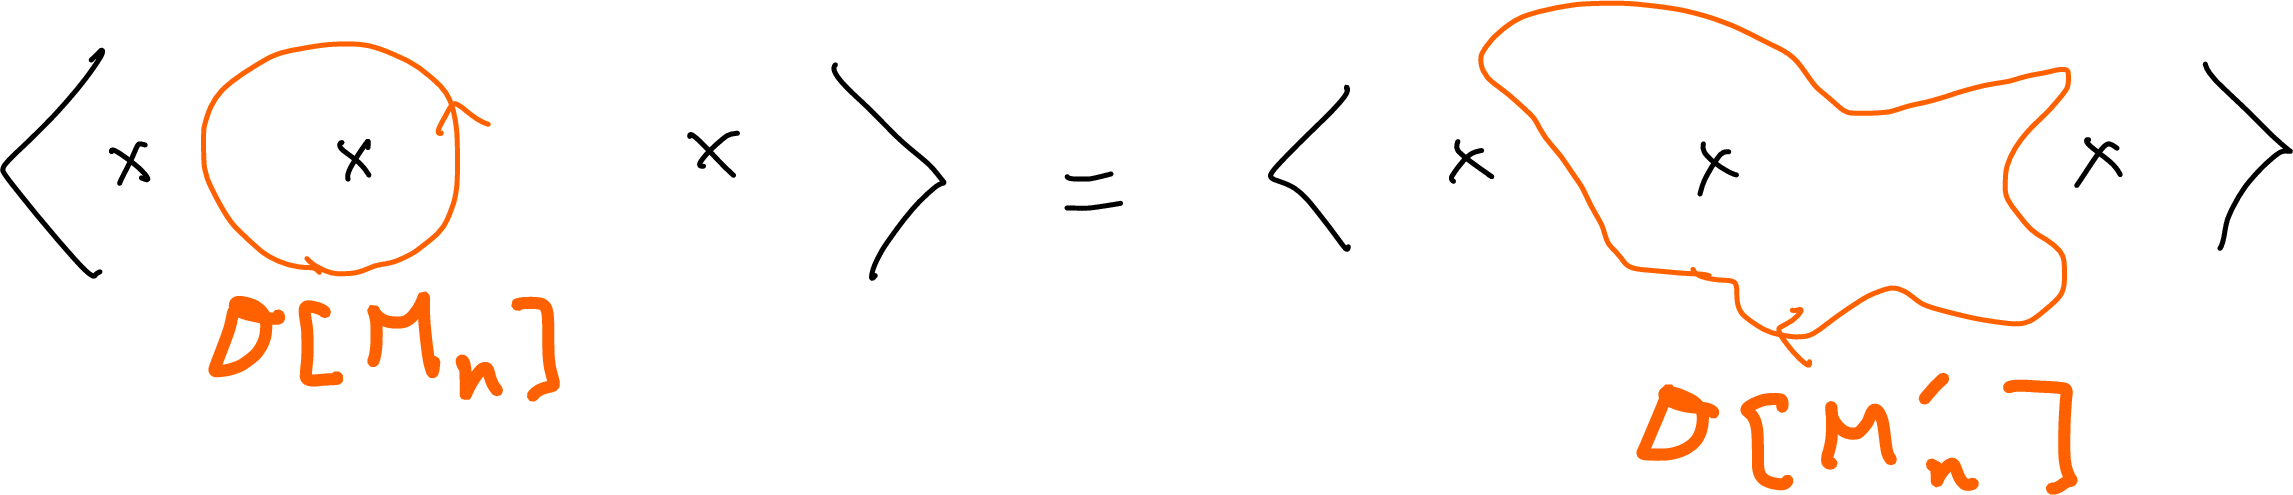
\includegraphics[width=4.16667in,height=\textheight]{figures/TopOpsDeform.png}

}

\caption{\label{fig-TopOpsDeform}Topological operator.}

\end{figure}

The first aim of the lecture is to understand the correspondence, that
is

\begin{tcolorbox}[enhanced jigsaw, breakable, rightrule=.15mm, bottomtitle=1mm, opacityback=0, titlerule=0mm, leftrule=.75mm, colframe=quarto-callout-important-color-frame, opacitybacktitle=0.6, toptitle=1mm, coltitle=black, title=\textcolor{quarto-callout-important-color}{\faExclamation}\hspace{0.5em}{\textsf{Symmetry/Topological Operator Correspondence}}, arc=.35mm, colback=white, left=2mm, bottomrule=.15mm, toprule=.15mm, colbacktitle=quarto-callout-important-color!10!white]

\begin{equation}\protect\hypertarget{eq-conv-STO-corresp}{}{\begin{split}
&\text{(Conventional) locality-preserving symmetry} \\ 
&\Longleftrightarrow\;
\text{invertible topological operator of codimension 1.}
\end{split}
}\label{eq-conv-STO-corresp}\end{equation}

\end{tcolorbox}

In this correspondence, the topological operator shoould be regarded as
the generalization of the \textbf{Noether charge} into possibly discrete
symmetry. To be precise, we regard this correspondence as the right-hand
side \emph{defining} the left-hand side. We will explicitly check this
correspondence/definition reproduces the known symmetries in the case of
scalar field theory in Chapter~\ref{sec-scalar} and in the case of
abelian gauge theory in Chapter~\ref{sec-vector}. The case of fermion is
very interesting and crucial, but it will be remained to be worked out
by audiences/readers.

\begin{tcolorbox}[enhanced jigsaw, breakable, rightrule=.15mm, bottomtitle=1mm, opacityback=0, titlerule=0mm, leftrule=.75mm, colframe=quarto-callout-note-color-frame, opacitybacktitle=0.6, toptitle=1mm, coltitle=black, title=\textcolor{quarto-callout-note-color}{\faInfo}\hspace{0.5em}{\textsf{Terminology}}, arc=.35mm, colback=white, left=2mm, bottomrule=.15mm, toprule=.15mm, colbacktitle=quarto-callout-note-color!10!white]

Again, we are \emph{not} talking about gauge redundancy, which is
sometimes called local symmetry. Global symmetries one encounters in a
QFT textbook are all locality preserving.

\end{tcolorbox}

\begin{tcolorbox}[enhanced jigsaw, breakable, rightrule=.15mm, bottomtitle=1mm, opacityback=0, titlerule=0mm, leftrule=.75mm, colframe=quarto-callout-note-color-frame, opacitybacktitle=0.6, toptitle=1mm, coltitle=black, title=\textcolor{quarto-callout-note-color}{\faInfo}\hspace{0.5em}{\textsf{Terminology}}, arc=.35mm, colback=white, left=2mm, bottomrule=.15mm, toprule=.15mm, colbacktitle=quarto-callout-note-color!10!white]

Here is another unfortunate conflict of terminology. In the literature
(outside generalized symmetry literature), a ``topological defect''
refers to a dynamical object, or its trajectory viewed as an operator in
the IR theory, charg\textbf{ed} under a topological (higher) symmetry.
As an operator in the IR theory, it is \emph{not} a priori guaranteed to
be topological in the sense of Figure~\ref{fig-TopOpsDeform} . On the
other hand, in the generalized symmetry literature, ``topological defect
(operator)'' often means an extended operator that is itself
topological. In this lecture, in order to ease the confusion, we use the
term ``topological operator''.

\end{tcolorbox}

\hypertarget{generalized-symmetry}{%
\section{Generalized Symmetry}\label{generalized-symmetry}}

The correspondence in Equation~\ref{eq-conv-STO-corresp} is the core in
the notion of \textbf{generalized (global) symmetry}, coined by
\autocite{Gaiotto:2014kfa} \footnote{The global higher-form symmetry
  itself had appeared and investigated in the literature,
  e.g.~\autocite{Kapustin:2013uxa,Barkeshli:2014cna}, and its gauged
  version was essentially known from \autocite{KalbRamond}.}. That is,
the notion of symmetry can be generalized by relaxing the adjective in
the right-hand side of Equation~\ref{eq-conv-STO-corresp}. Therefore, we
\emph{define} generalized symmetry by the following correspondence
generalizing Equation~\ref{eq-conv-STO-corresp}:

\begin{tcolorbox}[enhanced jigsaw, breakable, rightrule=.15mm, bottomtitle=1mm, opacityback=0, titlerule=0mm, leftrule=.75mm, colframe=quarto-callout-important-color-frame, opacitybacktitle=0.6, toptitle=1mm, coltitle=black, title=\textcolor{quarto-callout-important-color}{\faExclamation}\hspace{0.5em}{\textsf{Generalized Symmetry/Topological Operator Correspondence}}, arc=.35mm, colback=white, left=2mm, bottomrule=.15mm, toprule=.15mm, colbacktitle=quarto-callout-important-color!10!white]

\begin{equation}\protect\hypertarget{eq-GSTO-corresp}{}{\begin{split}
&\text{Generalized symmetry (in a ``usual" QFT)} \\ 
&\stackrel{\text{def}}{\Longleftrightarrow}\;
\text{General topological operator.}
\end{split}
}\label{eq-GSTO-corresp}\end{equation}

\end{tcolorbox}

More specifically, a generalized symmetry corresponding to an operator
of codimension \(p+1\) is called \textbf{\(p\)-form symmetry}, and a
generalized symmetry corresponding to an operator without its inverse is
called \textbf{non-invertible symmetry} (among other names like category
symmetry and topological symmetry).

In an ``unusual'' QFT, we can even relax the topological-ness of the
operator in the right-hand side of Equation~\ref{eq-GSTO-corresp},
resulting in what is called \textbf{subsystem} symmetry. We will briefly
make a comment on it in \textbf{?@sec-somewhere}.

The sub-classes of generalized symmetry is summarized in the table
below:

\begin{longtable}[]{@{}llll@{}}
\toprule\noalign{}
& \(p\)-form & non-invertible & subsystem \\
\midrule\noalign{}
\endhead
\bottomrule\noalign{}
\endlastfoot
codimension & \(p+1\) & & \\
Invertible? & & No & \\
Topological? & & & Partically \\
\end{longtable}

The subclasses are not mutually exclusive, so, in principle, there can
be a 2-form non-invertible subsystem symmetry.

\bookmarksetup{startatroot}

\hypertarget{sec-scalar}{%
\chapter{Topological Operators in Scalar Field
Theory}\label{sec-scalar}}

In this section we take a scalar field theory as an example to study
topological operators.

\hypertarget{scalar-transformation}{%
\section{Scalar Transformation}\label{scalar-transformation}}

\hypertarget{set-up}{%
\subsection{Set Up}\label{set-up}}

To be concrete, let us consider a complex scalar field theory whose
Lagrangian (density) on a spacetime of dimension \(\stdim\) is \[
\begin{aligned}
\mathcal{L}(\phi) &=  - \left(\frac12 \partial_\mu \phi(x)^* \partial^\nu \phi(x) + V(\phi(x))\right)\vol\\
&= \frac{1}{2} \mathop{d\phi} \wedge *\mathop{d\phi} - V(\phi(x))\vol,
\end{aligned}
\] where \(\vol = \prod_{i=1}^{\stdim} \mathop{dx_i}\) is the volume
form for the flat space, and \(V(\phi)\) is the potential. The action is
the integral over the spacetime \(M\): \[
S[\phi] = \int_{M}\mathcal{L}(\phi).
\]

We consider a symmetry transformation of the scalar field
\begin{equation}\protect\hypertarget{eq-scalar-transf}{}{
\phi(x) \mapsto \phi^g(x)
}\label{eq-scalar-transf}\end{equation} parametrized by a group element
\(g\) (constant over \(M\)) that leaves the action invariant:
\begin{equation}\protect\hypertarget{eq-action-inv}{}{
S[\phi]=S[\phi^g].
}\label{eq-action-inv}\end{equation} This means that the Lagrangian is
invariant up to a total derivative:
\begin{equation}\protect\hypertarget{eq-Lagrangian-inv}{}{
\mathcal{L}(\phi^g) = \mathcal{L}(\phi) + \mathop{ds}(\phi,g) 
}\label{eq-Lagrangian-inv}\end{equation} where \(s(\phi,g)\) is a
\((\stdim-1)\)-form on \(M\) depending on the constant \(g\) and the
field \(\phi\).

For example, the usual \(\U(1)\) rotation corresponds to the
transformation \[
\phi^g(x) = \mathop{g} \phi(x),
\] where \(g=e^{\imunit \alpha}\) is a \(\U(1)\) phase. The potential
\(V(\phi)\) might partially break the \(\U(1)\) rotation into its
subgroup \(\mathbb{Z}_k\), e.g.~\(V(\phi)\propto \phi^k+(\phi^*)^k\). In
such a case the parameter \(g\) takes \emph{discrete} values:
\(g = e^{\imunit \frac{2\pi i}{k}}\), \(i= 0 \cdots k-1\).

In addition, when \(V(\phi)=0\), the action \(S[\phi]\) also admit the
shift symmetry\footnote{If we use the form of Lagrangian
  \(\mathcal{L}^\prime= -\frac12 \phi \mathop{d*d\phi}\), this also
  gives an example where the total derivative in
  Equation~\ref{eq-Lagrangian-inv} is nonzero:
  \(r=-\frac12 \alpha \mathop{*}\mathop{d\phi}\).} \[
\phi^{\alpha}(x) = \phi(x) + \alpha.
\]

In this section, we would like to construct the \textbf{topological
operator} corresponding to this kind of (very conventional) symmetry.

\begin{tcolorbox}[enhanced jigsaw, breakable, rightrule=.15mm, bottomtitle=1mm, opacityback=0, titlerule=0mm, leftrule=.75mm, colframe=quarto-callout-note-color-frame, opacitybacktitle=0.6, toptitle=1mm, coltitle=black, title=\textcolor{quarto-callout-note-color}{\faInfo}\hspace{0.5em}{\textsf{Note}}, arc=.35mm, colback=white, left=2mm, bottomrule=.15mm, toprule=.15mm, colbacktitle=quarto-callout-note-color!10!white]

The construction will apply to other types of scalar field theory,
e.g.~real and/or multiple scalar fields, or a non-linear sigma model as
long as the kinetic term is standard enough (more on this in
\textbf{?@sec-somewhere}). Also, the spacetime manifold \(M\) and the
metric on it do not have to be flat. The signature of the metric is also
insignificant in this lecture, although we use the Euclidean notation.

\end{tcolorbox}

\begin{tcolorbox}[enhanced jigsaw, breakable, rightrule=.15mm, bottomtitle=1mm, opacityback=0, titlerule=0mm, leftrule=.75mm, colframe=quarto-callout-note-color-frame, opacitybacktitle=0.6, toptitle=1mm, coltitle=black, title=\textcolor{quarto-callout-note-color}{\faInfo}\hspace{0.5em}{\textsf{Note}}, arc=.35mm, colback=white, left=2mm, bottomrule=.15mm, toprule=.15mm, colbacktitle=quarto-callout-note-color!10!white]

In this lecture we directly construct the topological operators
corresponding to the \emph{finite} transformation
Equation~\ref{eq-scalar-transf}, rather than the conventional approach
that goes through the Noether's theorem. This will enable us to
explicitly talk about \emph{finite} symmetries (and their anomalies) in
terms of topological operators, and also motivate us the later sections.

\end{tcolorbox}

\hypertarget{topological-operator}{%
\subsection{Topological Operator}\label{topological-operator}}

As a basic example of Equation~\ref{eq-conv-STO-corresp}, we would like
to construct the topological operator \(U_\alpha[W]\) corresponding to
the transformation Equation~\ref{eq-scalar-transf}. The topological
operator \(U_\alpha[W]\) ,defined with respect to a codimension-1
submanifold \(W\) of the spacetime \(M\), should satisfy the following
properties:

\begin{tcolorbox}[enhanced jigsaw, breakable, rightrule=.15mm, bottomtitle=1mm, opacityback=0, titlerule=0mm, leftrule=.75mm, colframe=quarto-callout-important-color-frame, opacitybacktitle=0.6, toptitle=1mm, coltitle=black, title=\textcolor{quarto-callout-important-color}{\faExclamation}\hspace{0.5em}{\textsf{Properties of Symmetry Topological Operator}}, arc=.35mm, colback=white, left=2mm, bottomrule=.15mm, toprule=.15mm, colbacktitle=quarto-callout-important-color!10!white]

\begin{enumerate}
\def\labelenumi{\arabic{enumi}.}
\tightlist
\item
  Topological: \(U_\alpha[W] = U_\alpha[W']\) is \(W\) can be
  continuously defomed into \(W'\) without crossing other operators.
\item
  Symmetry action: when a deformation from \(W\) to \(W''\) crosses an
  local operator \(\mathcal{O}\), it gets the symmetry action specified
  by \(g\), resulting in another operator \(g\cdot\mathcal{O}\).
\end{enumerate}

These properties are summarized in Figure~\ref{fig-op-action}.

\end{tcolorbox}

\begin{figure}[t]

{\centering 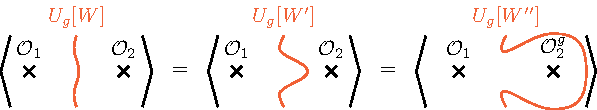
\includegraphics[width=4.16667in,height=\textheight]{index_files/mediabag/figures/Op_action.pdf}

}

\caption{\label{fig-op-action}The topological operator \(U_g[W]\) should
be invariant under a continuous deformation and also implement the
symmetry action.}

\end{figure}

The idea of the construction is
``\emph{cutting-and-gluing-with-twist}''. That is, we first divide the
spacetime \(M\) into two parts: \(M_\stdim = M_L \cup_W M_R\) with
shared boundary \(W\) (see Figure~\ref{fig-cut-M}). We also separate the
scalar field \(\phi\) into two sets of fields: \(\phi_L(x)\) for
\(x \in M_L\) and \(\phi_R(x)\) for \(x \in M_R\). Then, we glue the two
regions and fields on those back together, with the twisted
identification: \[
\phi_L|_W = \phi_R^g|_W.
\]

\begin{figure}[t]

{\centering 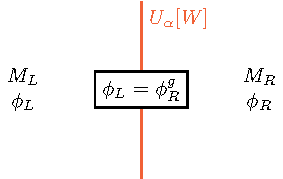
\includegraphics[width=2.39583in,height=\textheight]{index_files/mediabag/figures/ManifoldSplit.pdf}

}

\caption{\label{fig-cut-M}The cutting and twisted gluing, implementing
the topological operator \(U_g[W]\).}

\end{figure}

In path-integral, this construction can be implemented as follows:
\begin{equation}\protect\hypertarget{eq-Ug-pathintegral}{}{
\begin{multlined}
    \langle U_g[W] \cdots \rangle = \int \mathop{\mathcal{D}^{M_L}\phi_L} \mathop{\mathcal{D}^{M_R}\phi_R} \mathop{\mathcal{D}^W\lambda}\\ \times \exp\left(-S_L-S_R+\imunit \int_W \lambda(\phi_L - \phi_R^g)\vol_W+\int_W s(\phi_L,g)\right)\cdots
\end{multlined}
}\label{eq-Ug-pathintegral}\end{equation} Here, \(\mathcal{D}^{X}\)
denotes the measure for path-integral for a field defined on a
submanifold \(X\) of the spacetime \(M\), and
\(S_{L,R} = \int_{M_{L,R}}\mathcal{L}(\phi_{L,R})\) are actions on the
submanifold \(M_{L,R}\), and ``\(\cdots\)'' represents additional
insertions of operators. The heart of the above expression is that
integrating the Lagrange multiplier \(\lambda\) out gives the ``delta
functional'': \[
    \int \mathop{\mathcal{D}^W\lambda} \exp\left(\imunit \int_W \lambda (\phi_L-\phi^g_R)\vol_W\right)
     = \prod_{x\in W}\delta(\phi_L(x) - \phi_R^g(x)),
\] which should implement Figure~\ref{fig-cut-M}.

Let us check the property depicted in Figure~\ref{fig-op-action}. To be
concrete, we set the insertion \(\cdots\) to be
\(\mathcal{O}_1(x_1)\mathcal{O}_2(x_2)\) with \(x_1\in M_L\) and
\(x_2 \in M_R\).

\hypertarget{winding-symmetry-in-11d-compact-boson}{%
\section{Winding Symmetry in 1+1d Compact
Boson}\label{winding-symmetry-in-11d-compact-boson}}

\hypertarget{t-duality}{%
\section{T-duality}\label{t-duality}}

\bookmarksetup{startatroot}

\hypertarget{sec-vector}{%
\chapter{Vector}\label{sec-vector}}

\bookmarksetup{startatroot}

\hypertarget{summary}{%
\chapter{Summary}\label{summary}}

In summary, this book has no content whatsoever.

\bookmarksetup{startatroot}

\hypertarget{references}{%
\chapter*{References}\label{references}}
\addcontentsline{toc}{chapter}{References}

\markboth{References}{References}

\printbibliography[heading=none]




\end{document}
